\documentclass[11pt]{article}

\usepackage[margin=1in]{geometry}
\usepackage[T1]{fontenc}
\usepackage[utf8]{inputenc}
\usepackage{lmodern}
\usepackage{amsmath, amssymb, mathtools}
\usepackage{bm}
\usepackage{booktabs}
\usepackage{enumitem}
\usepackage{hyperref}
\usepackage{xcolor}
\usepackage{tikz}
\usetikzlibrary{arrows.meta, positioning}

\hypersetup{
    colorlinks=true,
    linkcolor=blue!50!black,
    urlcolor=blue!50!black,
    citecolor=blue!50!black
}

\setlist[itemize]{topsep=4pt,itemsep=2pt,parsep=0pt}
\setlist[enumerate]{topsep=4pt,itemsep=2pt,parsep=0pt}

\newcommand{\R}{\mathbb{R}}
\newcommand{\softmax}{\operatorname{softmax}}
\newcommand{\trans}{\mathsf{T}}

\title{FlashAttention-2 Deep Dive}
\author{}
\date{}

\begin{document}

\maketitle

\section{Purpose}

This document is a bottom-up study of FlashAttention-2 (FA2), with an emphasis
on how the attention equations map to CuTe/CUTLASS kernel structure, shared
memory layouts, warp-level tensor-core instructions, and the online softmax
update used in fused attention kernels.

Rather than starting from the full production kernel, we begin with a concrete
example and use it as a running study case throughout the rest of the document.

\section{Running Study Case}

We use the following self-attention configuration as our reference example:

\begin{itemize}
    \item batch size: $b = 1$
    \item sequence length: $\mathrm{seqlen} = 1024$
    \item number of heads: $n_{\mathrm{heads}} = 4$
    \item head dimension: $d = 128$
\end{itemize}

Therefore, the query, key, and value tensors have shape
\[
Q, K, V \in \R^{1 \times 4 \times 1024 \times 128}.
\]

For the purpose of this deep dive, we will often focus on a single head at a
time. In that view, the per-head tensors are
\[
Q_h, K_h, V_h \in \R^{1024 \times 128}.
\]

\subsection{Attention Math for One Head}

For a single head, the attention computation is
\begin{align}
S &= Q_h K_h^\trans, \\
P &= \softmax\!\left(\frac{S}{\sqrt{d}}\right), \\
O &= P V_h.
\end{align}

The tensor shapes are:
\begin{align}
Q_h, K_h, V_h &\in \R^{1024 \times 128}, \\
S &\in \R^{1024 \times 1024}, \\
P &\in \R^{1024 \times 1024}, \\
O &\in \R^{1024 \times 128}.
\end{align}


\subsection{A Simplified GPU Mapping Assumption}

As a first teaching model, we may assume that different heads are launched as
different CTAs, so one CTA handles tensors shaped like
\[
(1, 1, 1024, 128)
\]
for one head. This is a useful mental model for understanding the kernel
building blocks:

\begin{itemize}
    \item global-memory tiled copies,
    \item shared-memory layout and swizzle,
    \item \texttt{ldmatrix} loads,
    \item warp-level tensor-core MMA instructions,
    \item and the fusion of $QK^\trans$, softmax, and $PV$.
\end{itemize}

\paragraph{Why this is only a teaching model.}
Production FA2 kernels are usually tiled more finely than ``one CTA per head''.
In practice, a CTA typically owns a tile of query rows and streams over
many key/value tiles, while maintaining online softmax statistics. Still, the
single-head view is the right starting point for understanding the math and the
kernel microstructure.

\paragraph{Production mapping versus teaching model.}
It is helpful to distinguish the following execution scenarios:

\begin{itemize}
    \item \textbf{One CTA per head:} the whole head is owned by one CTA.
    \item \textbf{FA2 production tiling:} many CTAs can work on the same head,
    with each CTA responsible for a different tile.
\end{itemize}

In forward prefill or training, that tile is typically a block of query rows.
In the backward pass, the FA2 paper describes parallelizing by column blocks.
In decode, the mapping can change again because the query length is tiny and KV
loading becomes the main bottleneck.

\paragraph{Working execution model for this document.}
For the rest of this deep dive, we will adopt the simplified execution model
\[
\text{1 head} = \text{1 CTA}
\]
as our running assumption. In other words, one CTA owns
\[
Q_h, K_h, V_h \in \R^{1024 \times 128}
\]
for one head and computes the corresponding output
\[
O_h \in \R^{1024 \times 128}.
\]

This does \emph{not} mean the CTA computes attention as one giant monolithic
matrix multiply. The CTA still performs blocked computation internally. Using
the study tile sizes
\[
\mathrm{BlockM} = 64, \qquad \mathrm{BlockN} = 64, \qquad \mathrm{BlockK} = 64,
\]
the CTA conceptually executes three nested levels of work:

\begin{enumerate}
    \item split the query rows into $1024 / 64 = 16$ query-row tiles,
    \item for each query-row tile, stream over $1024 / 64 = 16$ key/value
    tiles,
    \item for each score-tile multiply, split the head dimension
    $128 = 64 + 64$ into two $\mathrm{BlockK}$ slices.
\end{enumerate}

So even under the ``1 head = 1 CTA'' simplification, the CTA still computes
attention tile by tile:
\begin{align}
S_{ij} &= Q_i K_j^\trans, \qquad S_{ij} \in \R^{64 \times 64}, \\
O_i &\leftarrow \text{online-softmax-update}(O_i, S_{ij}, V_j),
\end{align}
where:
\begin{itemize}
    \item $Q_i \in \R^{64 \times 128}$ is one query-row tile,
    \item $K_j, V_j \in \R^{64 \times 128}$ are one key/value tile pair,
    \item $O_i \in \R^{64 \times 128}$ is the output tile for those query rows.
\end{itemize}

This is the model we will use when discussing \texttt{kernel\_trait.h},
global-memory tiled copy, shared-memory layout, \texttt{ldmatrix}, and tensor
core MMA.

\subsection{How We Tile \texorpdfstring{$Q$, $K$, and $V$}{Q, K, and V}}

In the simplified kernel studied in this document, we use the tile sizes
\[
kBlockM = 64, \qquad kBlockN = 64, \qquad kBlockKSmem = 64.
\]

The intended shared-memory staging is:
\begin{itemize}
    \item tile $Q$ into blocks of shape
    \[
    kBlockM \times kBlockKSmem = 64 \times 64,
    \]
    \item tile $K$ into blocks of shape
    \[
    kBlockN \times kBlockKSmem = 64 \times 64,
    \]
    \item tile $V$ into blocks of shape
    \[
    kBlockN \times kBlockKSmem = 64 \times 64.
    \]
\end{itemize}

Since
\[
Q_h, K_h, V_h \in \R^{1024 \times 128},
\]
the sequence dimension is split into
\[
\mathrm{seqlen} / kBlockM = 1024 / 64 = 16
\]
tiles, and the head dimension is split into
\[
d / kBlockKSmem = 128 / 64 = 2
\]
slices.

\paragraph{Tiling of $Q$.}
We write the query matrix as
\[
Q_h =
\begin{bmatrix}
Q_0 \\
Q_1 \\
\vdots \\
Q_{15}
\end{bmatrix},
\qquad
Q_i \in \R^{64 \times 128}.
\]
Each query-row tile is then split along the head dimension:
\[
Q_i = \begin{bmatrix} Q_i^{(0)} & Q_i^{(1)} \end{bmatrix},
\qquad
Q_i^{(t)} \in \R^{64 \times 64},
\qquad
t \in \{0,1\}.
\]
So the actual shared-memory tile loaded for one inner MMA step is
\[
Q_i^{(t)} \in \R^{kBlockM \times kBlockKSmem}.
\]

\paragraph{Tiling of $K$.}
Similarly,
\[
K_h =
\begin{bmatrix}
K_0 \\
K_1 \\
\vdots \\
K_{15}
\end{bmatrix},
\qquad
K_j \in \R^{64 \times 128},
\]
and each key tile is split along the head dimension:
\[
K_j = \begin{bmatrix} K_j^{(0)} & K_j^{(1)} \end{bmatrix},
\qquad
K_j^{(t)} \in \R^{64 \times 64}.
\]
So one staged key tile for a single inner step is
\[
K_j^{(t)} \in \R^{kBlockN \times kBlockKSmem}.
\]

\paragraph{Tiling of $V$.}
The value matrix is tiled in the same way:
\[
V_h =
\begin{bmatrix}
V_0 \\
V_1 \\
\vdots \\
V_{15}
\end{bmatrix},
\qquad
V_j \in \R^{64 \times 128},
\]
with
\[
V_j = \begin{bmatrix} V_j^{(0)} & V_j^{(1)} \end{bmatrix},
\qquad
V_j^{(t)} \in \R^{64 \times 64}.
\]
So one staged value tile is
\[
V_j^{(t)} \in \R^{kBlockN \times kBlockKSmem}.
\]

\paragraph{What one score tile multiply looks like.}
For fixed query tile index $i$ and key tile index $j$, one score tile is
\[
S_{ij} = Q_i K_j^\trans \in \R^{64 \times 64}.
\]
Because the head dimension is split into two $64$-wide slices, this tile is
computed as
\[
S_{ij}
=
Q_i^{(0)} \left(K_j^{(0)}\right)^\trans
+
Q_i^{(1)} \left(K_j^{(1)}\right)^\trans.
\]

So pictorially, the CTA uses:
\begin{itemize}
    \item one $64 \times 64$ tile from $Q$,
    \item one $64 \times 64$ tile from $K$,
    \item and accumulates into one $64 \times 64$ score tile,
\end{itemize}
then repeats for the second head-dimension slice.

\paragraph{The \texorpdfstring{$QK^\trans$}{QK^T} GEMM main loop as a loop nest.}
At the CTA level, the tiled score computation can be viewed as the following
loop nest:

\begin{verbatim}
for i in 0 .. (seqlen / kBlockM) - 1:
  // Q_i is one query-row tile
  // Q_i has shape (kBlockM, d)

  for j in 0 .. (seqlen / kBlockN) - 1:
    // K_j is one key tile
    // K_j has shape (kBlockN, d)

    S_ij = 0
    // S_ij has shape (kBlockM, kBlockN)

    for t in 0 .. (d / kBlockKSmem) - 1:
      // Q_i^(t) has shape (kBlockM, kBlockKSmem)
      // K_j^(t) has shape (kBlockN, kBlockKSmem)

      load Q_i^(t)
      load K_j^(t)
      S_ij += Q_i^(t) @ (K_j^(t))^T
\end{verbatim}

Using the concrete study parameters
\[
\mathrm{seqlen} = 1024, \qquad d = 128, \qquad
kBlockM = kBlockN = kBlockKSmem = 64,
\]
this becomes:
\begin{itemize}
    \item $i = 0, \dots, 15$ for the $16$ query-row tiles,
    \item $j = 0, \dots, 15$ for the $16$ key tiles,
    \item $t = 0, 1$ for the $2$ head-dimension slices.
\end{itemize}

So one CTA computes the full score matrix by accumulating
\[
\frac{\mathrm{seqlen}}{kBlockM}
\times
\frac{\mathrm{seqlen}}{kBlockN}
=
16 \times 16 = 256
\]
score tiles, and each score tile is itself formed from
\[
\frac{d}{kBlockKSmem} = 2
\]
partial products.

\paragraph{What \texttt{GmemTiledCopyQKV} does.}
For a staged tile such as
\[
Q_i^{(t)} \in \R^{kBlockM \times kBlockKSmem},
\]
\texttt{GmemTiledCopyQKV} is the CTA-collective global-memory to shared-memory
copy object created by
\begin{quote}
\texttt{make\_tiled\_copy(Copy\_Atom<...>, GmemLayoutAtom, Layout<Shape<\_1,\_8>>)}
\end{quote}
Its three ingredients play different roles:
\begin{itemize}
    \item \texttt{Copy\_Atom<Gmem\_copy\_struct, Element>} chooses the atomic
    copy width. In our case, it is a $128$-bit gmem copy per thread
    (\texttt{cp.async} when enabled).
    \item \texttt{GmemLayoutAtom} arranges the CTA threads as a logical
    $16 \times 8$ thread array.
    \item \texttt{Layout<Shape<\_1,\_8>>} says that each thread's payload is
    interpreted as a $1 \times 8$ fragment of \texttt{Element}.
\end{itemize}

Since \texttt{Element = half}, one $128$-bit copy contains
\[
16 \text{ bytes} / 2 \text{ bytes per element} = 8
\]
elements. Therefore, one CTA-wide copy round covers a tile of shape
\[
16 \times 64.
\]

\paragraph{Question 1: how many \texttt{GmemTiledCopyQKV} rounds are needed for one staged $Q$ block?}
We focus on one staged query block
\[
Q_i^{(t)} \in \R^{64 \times 64}.
\]

\paragraph{Pictorially, what is the copy problem?}
At this stage, the CTA contains $4$ warps, so it has
\[
kNThreads = 4 \times 32 = 128
\]
threads in total. The problem is that these $128$ threads must collectively
load one staged $Q$ tile of shape
\[
64 \times 64
\]
from global memory into shared memory.

Since each thread copies one $128$-bit chunk, and \texttt{Element = half}, each
thread loads $8$ contiguous elements. So one row of width $64$ is naturally
split across
\[
64 / 8 = 8
\]
threads. Therefore, one CTA-wide round uses:
\begin{itemize}
    \item $8$ threads to cover each row,
    \item all $128$ threads to cover
    \[
    128 / 8 = 16
    \]
    rows at once.
\end{itemize}

So pictorially, one \texttt{GmemTiledCopyQKV} round covers a
\[
16 \times 64
\]
sub-tile of the full $64 \times 64$ staged $Q$ block. That is why the full
tile requires multiple rounds.

\paragraph{Derivation using the kernel symbols.}
From the code,
\[
kGmemElemsPerLoad
=
\frac{\text{sizeof(cute::uint128\_t)}}{\text{sizeof(Element)}}
=
\frac{16}{2}
=
8.
\]
So each thread copies $8$ elements. Next,
\[
kGmemThreadsPerRow
=
\frac{kBlockKSmem}{kGmemElemsPerLoad}
=
\frac{64}{8}
=
8,
\]
so $8$ threads cover one row. Since
\[
kNThreads = 4 \times 32 = 128,
\]
one copy round covers
\[
\frac{kNThreads}{kGmemThreadsPerRow}
=
\frac{128}{8}
=
16
\]
rows, i.e. a tile of shape
\[
16 \times 64.
\]
Therefore, the number of rounds needed for one $64 \times 64$ staged $Q$ block
is
\[
\frac{64 \times 64}{16 \times 64}
=
\frac{64}{16}
=
4.
\]

\paragraph{Equivalent byte-count derivation.}
The same answer can be obtained by counting bytes. One staged $Q$ block contains
\[
64 \times 64 \times 2 = 8192
\]
bytes. One CTA-wide copy round moves
\[
128 \text{ threads} \times 16 \text{ bytes per thread} = 2048
\]
bytes. Therefore,
\[
\frac{64 \times 64 \times 2}{128 \times 16}
=
\frac{8192}{2048}
=
4.
\]

\subsection{Mathematical Work Completed by One CTA}

Under the simplified execution model
\[
\text{1 head} = \text{1 CTA},
\]
one CTA is responsible for computing the entire attention output for one head:
\[
O_h = \softmax\!\left(\frac{Q_h K_h^\trans}{\sqrt{128}}\right)V_h,
\]
where
\[
Q_h, K_h, V_h \in \R^{1024 \times 128},
\qquad
O_h \in \R^{1024 \times 128}.
\]

So, mathematically, one CTA must complete three tasks for that head:
\begin{enumerate}
    \item compute all attention scores
    \[
    S_h = Q_h K_h^\trans \in \R^{1024 \times 1024},
    \]
    \item compute the row-wise softmax
    \[
    P_h = \softmax\!\left(\frac{S_h}{\sqrt{128}}\right)
    \in \R^{1024 \times 1024},
    \]
    \item compute the final output
    \[
    O_h = P_h V_h \in \R^{1024 \times 128}.
    \]
\end{enumerate}

\paragraph{Row-wise view.}
Equivalently, for each query row $r$, the CTA must compute:
\begin{align}
s_r &= q_r K_h^\trans \in \R^{1024}, \\
p_r &= \softmax\!\left(\frac{s_r}{\sqrt{128}}\right) \in \R^{1024}, \\
o_r &= p_r V_h \in \R^{128}.
\end{align}

Here, $q_r \in \R^{128}$ is the $r$-th row of $Q_h$, $s_r$ is the score vector
for that row, $p_r$ is the probability vector, and $o_r$ is the output row.

\paragraph{Blocked view with the study tile sizes.}
Using
\[
\mathrm{BlockM} = 64, \qquad \mathrm{BlockN} = 64, \qquad \mathrm{BlockK} = 64,
\]
we partition the head into:
\begin{itemize}
    \item $16$ query-row tiles
    \[
    Q_i \in \R^{64 \times 128}, \qquad i = 0, \dots, 15,
    \]
    \item $16$ key/value tiles
    \[
    K_j, V_j \in \R^{64 \times 128}, \qquad j = 0, \dots, 15.
    \]
\end{itemize}

For each fixed query tile $Q_i$, the CTA maintains three pieces of running
state:
\begin{itemize}
    \item a running row max
    \[
    m_i \in \R^{64},
    \]
    \item a running row sum
    \[
    l_i \in \R^{64},
    \]
    \item and a running output tile
    \[
    O_i \in \R^{64 \times 128}.
    \]
\end{itemize}

For each key/value tile index $j$, the CTA computes the score tile
\[
S_{ij} = Q_i K_j^\trans \in \R^{64 \times 64}.
\]

Because the head dimension is
\[
128 = 64 + 64,
\]
this tile is itself formed from two partial products along the reduction
dimension:
\[
S_{ij}
=
Q_i^{(0)} \left(K_j^{(0)}\right)^\trans
+
Q_i^{(1)} \left(K_j^{(1)}\right)^\trans,
\]
where each partial operand has shape
\[
Q_i^{(t)}, K_j^{(t)} \in \R^{64 \times 64},
\qquad
t \in \{0,1\}.
\]

After computing $S_{ij}$, the CTA scales it:
\[
\widehat{S}_{ij} = \frac{S_{ij}}{\sqrt{128}}.
\]

The CTA then performs an online softmax update. Let
\[
m_{ij} = \operatorname{rowmax}(\widehat{S}_{ij}) \in \R^{64}.
\]
Then the updated running row max is
\[
m_i' = \max(m_i, m_{ij}).
\]

Define the unnormalized probability tile
\[
\widetilde{P}_{ij} = \exp\!\left(\widehat{S}_{ij} - m_i'\right)
\in \R^{64 \times 64},
\]
where the vector $m_i'$ is broadcast across columns.

The running row sum is updated by
\[
l_i' = e^{m_i - m_i'} \odot l_i + \operatorname{rowsum}(\widetilde{P}_{ij}),
\]
where $\odot$ is elementwise multiplication.

Finally, the output tile is updated by combining the rescaled old output with
the new contribution from $V_j$:
\[
O_i'
=
\frac{
\operatorname{diag}\!\left(e^{m_i - m_i'} \odot l_i\right) O_i
+
\widetilde{P}_{ij} V_j
}{
\operatorname{diag}(l_i')
}.
\]

Then the CTA advances its running state:
\[
(m_i, l_i, O_i) \leftarrow (m_i', l_i', O_i').
\]

After iterating over all $j = 0, \dots, 15$ for every query tile $i = 0, \dots,
15$, the concatenation of all output tiles $O_i$ gives the full head output
$O_h$.

\section{Why This Example Is Useful}

This study case is large enough to expose the core FA2 ideas:

\begin{itemize}
    \item the score matrix $S$ is too large to materialize cheaply for every
    head,
    \item tensor-core kernels naturally operate on tiles rather than full
    matrices,
    \item the softmax must be computed in a numerically stable streaming form,
    \item and the dataflow must be organized around global memory, shared
    memory, registers, and warp-level MMA fragments.
\end{itemize}

At the same time, the example is still small enough that every dimension is easy
to reason about by hand:

\begin{itemize}
    \item the reduction dimension is $d = 128$,
    \item the sequence dimension is $1024$,
    \item and both are divisible by the common study tile size $64$.
\end{itemize}

\section{How We Will Use This Example Later}

In later sections, we will revisit this same study case to answer a sequence of
kernel questions:

\begin{enumerate}
    \item How many rounds of global-memory tiled copy are needed for one block?
    \item What exactly does \texttt{ldmatrix} load into each lane?
    \item Why is a shared-memory swizzle needed, and why does
    \texttt{Swizzle<3,3,3>} show up so often?
    \item What does one tensor-core MMA atom compute?
    \item Why can the same MMA machinery support both $QK^\trans$ and $PV$?
    \item How does FA2 avoid materializing the full score and probability
    matrices?
    \item How does the online softmax recurrence make the fusion numerically
    stable?
\end{enumerate}


\section{RL Training and Backward Pass Context}

Although the running study case above uses a dense single-sequence forward
pass, later discussion will also connect FlashAttention-2 to RL training
workloads and the backward pass. In that setting, the relevant forward API is
often the packed varlen path, where each sample is a causal sequence of the
form $[\text{prompt};\text{response}]$. The figure below gives the forward-side
picture that motivates that later discussion.

\subsection{Pictorial View of Packed Varlen Forward}

In RL training, one batch often contains several causal sequences of the form
$[\text{prompt};\text{response}]$. The varlen FlashAttention interface packs all
real tokens into one linearized $q/k/v$ buffer, while $\texttt{cu\_seqlens}$ records
where each sequence begins and ends.

\begin{figure}[ht]
    \centering
    \footnotesize
    \resizebox{\textwidth}{!}{%
    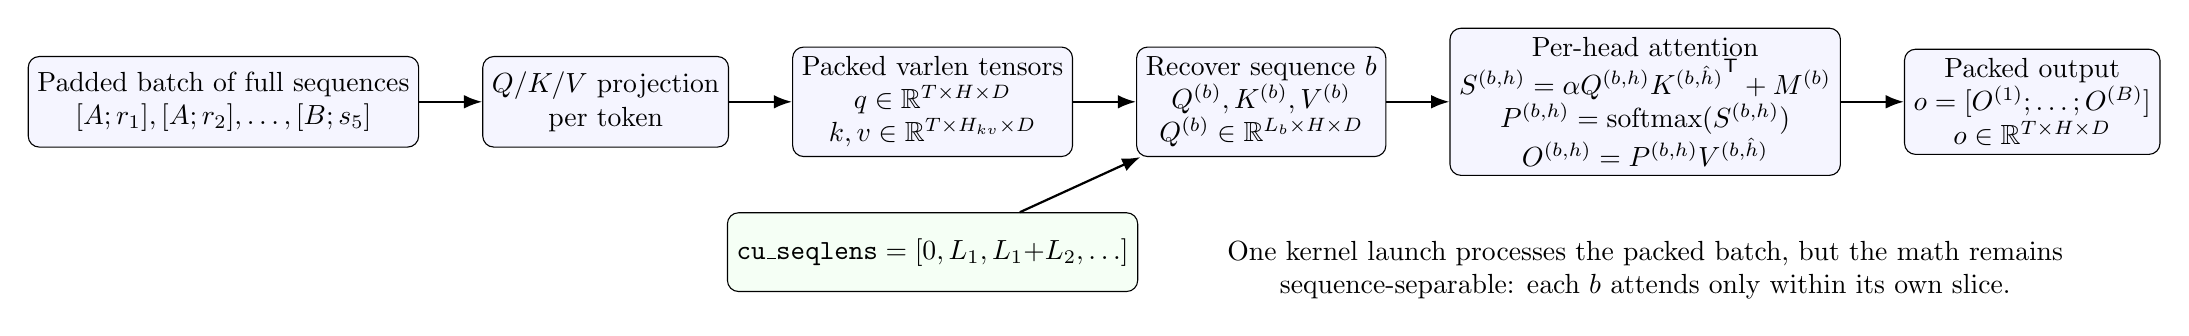
\begin{tikzpicture}[
        >=Latex,
        box/.style={draw, rounded corners, align=center, minimum height=1.15cm, minimum width=2.8cm, fill=blue!4},
        smallbox/.style={draw, rounded corners, align=center, minimum height=1.0cm, minimum width=2.9cm, fill=green!4},
        note/.style={align=center}
    ]
        \node[box] (batch) {Padded batch of full sequences\\$[A;r_1], [A;r_2], \ldots, [B;s_5]$};
        \node[box, right=8mm of batch] (proj) {$Q/K/V$ projection\\per token};
        \node[box, right=8mm of proj] (pack) {Packed varlen tensors\\$q \in \R^{T \times H \times D}$\\$k,v \in \R^{T \times H_{kv} \times D}$};
        \node[smallbox, below=7mm of pack] (cuseq) {$\texttt{cu\_seqlens}=[0,L_1,L_1{+}L_2,\ldots]$};
        \node[box, right=8mm of pack] (slice) {Recover sequence $b$\\$Q^{(b)},K^{(b)},V^{(b)}$\\$Q^{(b)} \in \R^{L_b \times H \times D}$};
        \node[box, right=8mm of slice] (math) {Per-head attention\\$S^{(b,h)} = \alpha Q^{(b,h)} {K^{(b,\hat h)}}^\trans + M^{(b)}$\\$P^{(b,h)} = \softmax(S^{(b,h)})$\\$O^{(b,h)} = P^{(b,h)} V^{(b,\hat h)}$};
        \node[box, right=8mm of math] (out) {Packed output\\$o=[O^{(1)};\ldots;O^{(B)}]$\\$o \in \R^{T \times H \times D}$};

        \draw[->, thick] (batch) -- (proj);
        \draw[->, thick] (proj) -- (pack);
        \draw[->, thick] (pack) -- (slice);
        \draw[->, thick] (slice) -- (math);
        \draw[->, thick] (math) -- (out);
        \draw[->, thick] (cuseq) -- (slice);

        \node[note, below=7mm of math] (note) {One kernel launch processes the packed batch, but the math remains\\sequence-separable: each $b$ attends only within its own slice.};
    \end{tikzpicture}%
    }
    \caption{Packed varlen forward pass used by \texttt{FlashAttnVarlenFunc.forward}. Padding is removed before the kernel launch, while $\texttt{cu\_seqlens}$ preserves per-sequence boundaries inside the packed $q/k/v$ tensors.}
\end{figure}




\paragraph{Mathematical Formula.}

Let
\[
q \in \R^{T \times H \times D}, \qquad
k, v \in \R^{T \times H_{kv} \times D},
\]
and let the packed sequence boundaries be given by
\[
\texttt{cu\_seqlens}[0] = 0, \qquad
\texttt{cu\_seqlens}[b+1] = \texttt{cu\_seqlens}[b] + L_b.
\]
For sequence $b$, the packed forward pass first recovers the per-sequence
slices
\[
Q^{(b)} = q[\texttt{cu\_seqlens}[b] : \texttt{cu\_seqlens}[b+1]]
\in \R^{L_b \times H \times D},
\]
\[
K^{(b)} = k[\texttt{cu\_seqlens}[b] : \texttt{cu\_seqlens}[b+1]], \qquad
V^{(b)} = v[\texttt{cu\_seqlens}[b] : \texttt{cu\_seqlens}[b+1]]
\in \R^{L_b \times H_{kv} \times D}.
\]
For one query head $h$ and its associated KV head $\hat h$, FlashAttention
then computes
\[
S^{(b,h)} = \alpha Q^{(b,h)} {K^{(b,\hat h)}}^\trans + M^{(b)}
\in \R^{L_b \times L_b},
\]
\[
P^{(b,h)} = \softmax\!\left(S^{(b,h)}\right)
\in \R^{L_b \times L_b},
\]
\[
O^{(b,h)} = P^{(b,h)} V^{(b,\hat h)}
\in \R^{L_b \times D},
\]
where $\alpha = 1 / \sqrt{D}$ in the standard scaled-dot-product case and
$M^{(b)}$ is the causal or local mask for sequence $b$.

Collecting all heads gives
\[
O^{(b)} \in \R^{L_b \times H \times D},
\]
and collecting all sequences back into packed form gives the final output
\[
o = [O^{(1)}; O^{(2)}; \ldots; O^{(B)}] \in \R^{T \times H \times D}.
\]
Thus, the varlen API executes one packed kernel launch, but mathematically it
still performs attention independently on each recovered sequence slice.

\subsection{Pictorial View of Packed Varlen Backward}

The backward pass for \texttt{FlashAttnVarlenFunc} starts from the upstream
output gradient
\[
dO = \frac{\partial L}{\partial O}
\in \R^{T \times H \times D},
\]
plus the tensors saved from the forward pass:
\[
q \in \R^{T \times H \times D}, \qquad
k,v \in \R^{T \times H_{kv} \times D}, \qquad
out \in \R^{T \times H \times D},
\]
\[
\texttt{softmax\_lse} \in \R^{H \times T}, \qquad
\texttt{cu\_seqlens\_q}, \texttt{cu\_seqlens\_k} \in \mathbb{Z}^{B+1}.
\]
The kernels reconstruct per-sequence slices, recompute the local attention
probabilities, and then form all gradients needed by the surrounding
transformer block.

\begin{figure}[ht]
    \centering
    \scriptsize
    \resizebox{\textwidth}{!}{%
    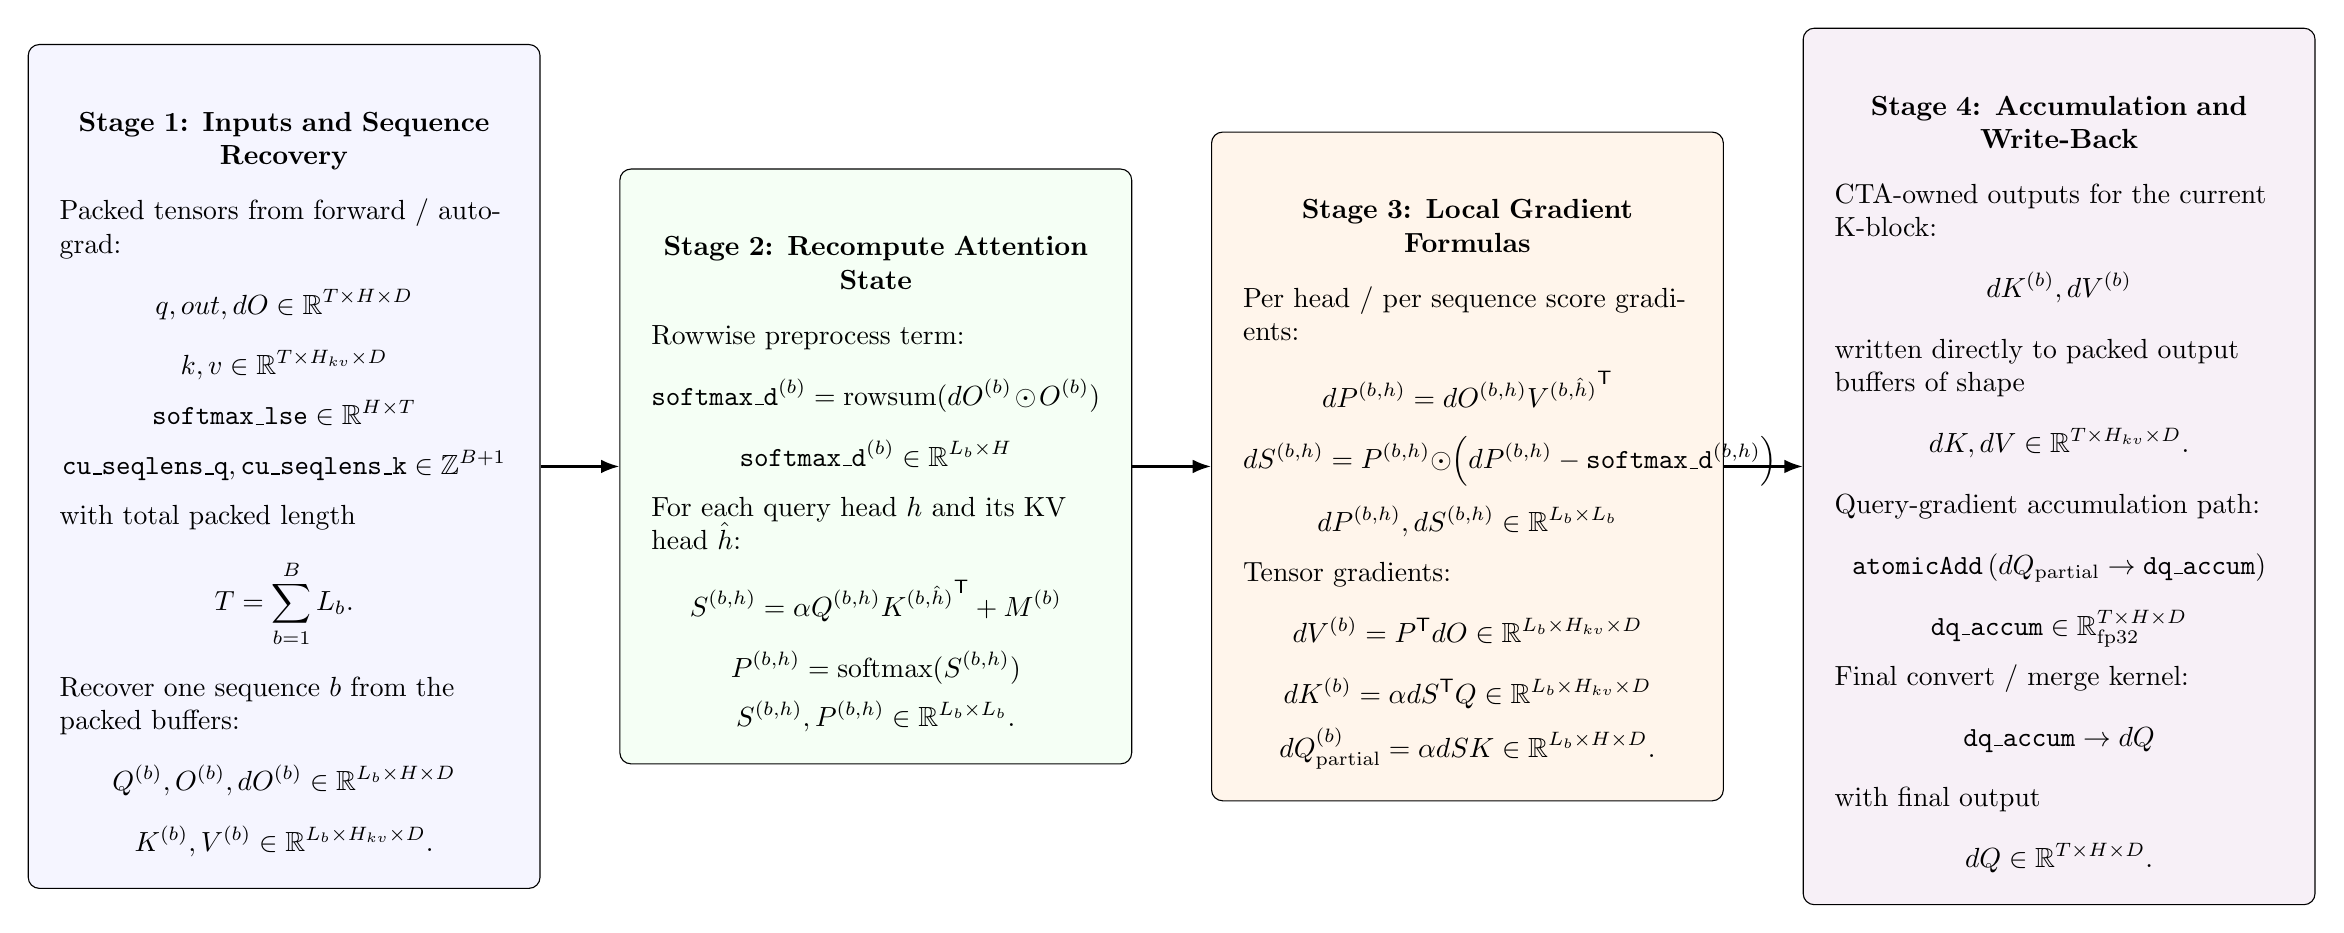
\begin{tikzpicture}[
        >=Latex,
        stage/.style={draw, rounded corners, align=left, minimum height=7.1cm, text width=5.7cm, inner sep=4mm},
        stageblue/.style={stage, fill=blue!4},
        stagegreen/.style={stage, fill=green!4},
        stageorange/.style={stage, fill=orange!8},
        stageviolet/.style={stage, fill=violet!6},
        flow/.style={->, thick}
    ]
        \node[stageblue] (inputs) at (0,0) {
            \begin{center}\textbf{Stage 1: Inputs and Sequence Recovery}\end{center}
            Packed tensors from forward / autograd:
            \[
            q, out, dO \in \R^{T \times H \times D}
            \]
            \[
            k, v \in \R^{T \times H_{kv} \times D}
            \]
            \[
            \texttt{softmax\_lse} \in \R^{H \times T}
            \]
            \[
            \texttt{cu\_seqlens\_q}, \texttt{cu\_seqlens\_k} \in \mathbb{Z}^{B+1}
            \]
            with total packed length
            \[
            T = \sum_{b=1}^{B} L_b.
            \]
            Recover one sequence $b$ from the packed buffers:
            \[
            Q^{(b)}, O^{(b)}, dO^{(b)} \in \R^{L_b \times H \times D}
            \]
            \[
            K^{(b)}, V^{(b)} \in \R^{L_b \times H_{kv} \times D}.
            \]
        };

        \node[stagegreen, right=10mm of inputs] (recompute) {
            \begin{center}\textbf{Stage 2: Recompute Attention State}\end{center}
            Rowwise preprocess term:
            \[
            \texttt{softmax\_d}^{(b)} = \operatorname{rowsum}(dO^{(b)} \odot O^{(b)})
            \]
            \[
            \texttt{softmax\_d}^{(b)} \in \R^{L_b \times H}
            \]
            For each query head $h$ and its KV head $\hat h$:
            \[
            S^{(b,h)} = \alpha Q^{(b,h)} {K^{(b,\hat h)}}^\trans + M^{(b)}
            \]
            \[
            P^{(b,h)} = \softmax(S^{(b,h)})
            \]
            \[
            S^{(b,h)}, P^{(b,h)} \in \R^{L_b \times L_b}.
            \]
        };

        \node[stageorange, right=10mm of recompute] (locals) {
            \begin{center}\textbf{Stage 3: Local Gradient Formulas}\end{center}
            Per head / per sequence score gradients:
            \[
            dP^{(b,h)} = dO^{(b,h)} {V^{(b,\hat h)}}^\trans
            \]
            \[
            dS^{(b,h)} = P^{(b,h)} \odot \left(dP^{(b,h)} - \texttt{softmax\_d}^{(b,h)}\right)
            \]
            \[
            dP^{(b,h)}, dS^{(b,h)} \in \R^{L_b \times L_b}
            \]
            Tensor gradients:
            \[
            dV^{(b)} = P^\trans dO \in \R^{L_b \times H_{kv} \times D}
            \]
            \[
            dK^{(b)} = \alpha dS^\trans Q \in \R^{L_b \times H_{kv} \times D}
            \]
            \[
            dQ_{\mathrm{partial}}^{(b)} = \alpha dS K \in \R^{L_b \times H \times D}.
            \]
        };

        \node[stageviolet, right=10mm of locals] (merge) {
            \begin{center}\textbf{Stage 4: Accumulation and Write-Back}\end{center}
            CTA-owned outputs for the current K-block:
            \[
            dK^{(b)}, dV^{(b)}
            \]
            written directly to packed output buffers of shape
            \[
            dK, dV \in \R^{T \times H_{kv} \times D}.
            \]
            Query-gradient accumulation path:
            \[
            \texttt{atomicAdd}\left(dQ_{\mathrm{partial}} \rightarrow \texttt{dq\_accum}\right)
            \]
            \[
            \texttt{dq\_accum} \in \R^{T \times H \times D}_{\mathrm{fp32}}
            \]
            Final convert / merge kernel:
            \[
            \texttt{dq\_accum} \rightarrow dQ
            \]
            with final output
            \[
            dQ \in \R^{T \times H \times D}.
            \]
        };

        \draw[flow] (inputs) -- (recompute);
        \draw[flow] (recompute) -- (locals);
        \draw[flow] (locals) -- (merge);
    \end{tikzpicture}%
    }
    \caption{Packed varlen backward pass used by \texttt{FlashAttnVarlenFunc.backward}. The diagram shows both the local per-sequence tensors with length $L_b$ and the packed global buffers with total length $T$, together with the shapes of every intermediate gradient object needed by the backward pass.}
\end{figure}



\subsection{Concrete Qwen3-8B GRPO Workload and Theoretical Latency}

To make the RL discussion concrete, consider end-to-end GRPO training on $4 \times 8$
A100 GPUs. The rollout generation phase and the policy-update phase are
\emph{time shared} across the same $32$ GPUs: during rollout they act as $32$
TP$=1$ vLLM replicas, and during the update they act as a $32$-way FSDP job.

\begin{table}[ht]
    \centering
    \small
    \begin{tabular}{ll}
        \toprule
        Setting & Value \\
        \midrule
        Algorithm & GRPO \\
        Model & \texttt{Qwen/Qwen3-8B} \\
        Data & Standard GSM8K \\
        Hardware & $4 \times 8$ A100 GPUs \\
        Nodes & 4 \\
        Total GPUs & 32 \\
        Rollout / update scheduling & Time shared across the same 32 GPUs \\
        TP during rollout & 2 \\
        Rollout replicas & 16 vLLM replicas \\
        Policy update parallelism & FSDP on 32 GPUs \\
        Prompt batch size & 32 unique prompts per RL step \\
        Training batch size & 256 sequences = 32 prompts $\times$ 8 rollouts \\
        Micro-batch size (policy update) & 8 sequences / GPU = 1 prompt group \\
        PPO mini-batch size & 256 \\
        Max prompt length & 8192 \\
        Max response length & 2048 \\
        Max total sequence length & 10240 \\
        Learning rate & $10^{-6}$ \\
        Optimizer offload & False \\
        Param offload & False (actor), True (ref) \\
        Gradient checkpointing & True \\
        Dtype & bf16 \\
        GPU memory utilization & 0.4 \\
        \bottomrule
    \end{tabular}
    \caption{Concrete long-context GRPO configuration used to reason about end-to-end RL latency on $32$ time-shared A100 GPUs.}
\end{table}

\paragraph{Notation and training-unit definitions.}
Here $N_p$ is the number of unique prompts drawn from the underlying training
dataset per RL step, $n$ is the number of sampled rollouts per prompt,
$B = N_p n$ is the \emph{training batch size} measured in prompt-response
trajectories for one policy update, $G$ is the total number of GPUs,
$\mathrm{TP}=2$ is the rollout tensor-parallel degree, and
$R = G / \mathrm{TP} = 16$ is the number of rollout replicas. In this
section, a \emph{step} means one end-to-end RL iteration: sample $N_p$ prompts,
generate $n$ rollouts per prompt, compute rewards and advantages, and run the
GRPO policy update on the resulting $B$ sequences. With $G=32$ GPUs in the
policy-update phase, the local micro-batch size is $B/G = 256/32 = 8$
sequences per GPU, which is exactly one prompt group. An \emph{epoch} means one
full pass over the underlying prompt dataset, so it is counted over prompts
rather than rollouts. If the dataset contains $N_{\mathrm{data}}$ prompts, then
the number of steps per epoch is approximately
\[
\left\lceil \frac{N_{\mathrm{data}}}{N_p} \right\rceil.
\]
For the GSM8K train split with $N_{\mathrm{data}} = 7473$, this gives about
$234$ steps per epoch (or $233$ with \texttt{drop\_last}).

\paragraph{Derived workload sizes.}
Let
\[
N_p = 32, \qquad n = 8, \qquad B = N_p n = 256, \qquad G = 32,
\]
\[
L_p = 8192, \qquad L_r = 2048, \qquad L = L_p + L_r = 10240.
\]
The full packed training batch therefore contains
\[
B L = 256 \times 10240 = 2{,}621{,}440
\]
tokens. Of these, the duplicated prompt portion is
\[
N_p n L_p = 32 \times 8 \times 8192 = 2{,}097{,}152,
\]
while the response portion is
\[
N_p n L_r = 32 \times 8 \times 2048 = 524{,}288.
\]
So in this workload, the prompt tokens account for
\[
\frac{L_p}{L} = \frac{8192}{10240} = 0.8
\]
of every training sequence.

\paragraph{Prompt-group placement under $\mathrm{TP}=2$.}
With rollout tensor parallelism $\mathrm{TP}=2$, the $32$ GPUs form
\[
R = \frac{G}{\mathrm{TP}} = \frac{32}{2} = 16
\]
rollout replicas. Since there are $N_p = 32$ prompt groups per RL step, each
rollout replica is responsible for
\[
\frac{N_p}{R} = \frac{32}{16} = 2
\]
prompt groups on average. During the policy update, however, the layout is still
especially clean because
\[
\frac{B}{G} = \frac{256}{32} = 8 = n.
\]
So if the training batch is laid out by prompt group, each GPU can still hold
exactly one GRPO prompt group of $8$ sibling rollouts. The local token budget
per GPU during the update is therefore
\[
nL = 8 \times 10240 = 81{,}920
\]
tokens. Relative to the earlier $24$-GPU setting, the $32$-GPU setup is still a
good match for grouped GRPO training, but rollout locality is now two prompt
groups per TP$=2$ replica rather than one prompt group per single-GPU replica.

\paragraph{Latency decomposition for one RL step.}
A useful step-level latency model is
\[
T_{\mathrm{RL\ step}}
\approx
T_{\mathrm{rollout}}(16, \mathrm{TP}=2)
+
T_{\mathrm{reward/advantage}}
+
T_{\mathrm{GRPO\ update}}(32)
+
T_{\mathrm{sync}}.
\]
Because rollout and update time-share the same $32$ GPUs, the practical
wall-clock lens is slightly different across the two phases: rollout is shaped
by the \emph{per-replica} local work of $16$ TP$=2$ replicas, while the update
is shaped by the \emph{per-GPU} local work of the $32$-way FSDP job. The long
shared prompt mainly affects the first and third terms:
\begin{itemize}
    \item \textbf{Rollout generation:} each TP$=2$ replica owns about two prompt
    groups, so rollout latency is well-approximated by twice the attention work
    of one prompt group under balanced sharding.
    \item \textbf{GRPO update:} if sibling rollouts remain colocated, then a
    future shared-prefix training kernel could still exploit one prompt group per
    GPU during the policy update.
\end{itemize}

\paragraph{Attention-only rollout proxy without sharing.}
For one prompt group of $8$ rollouts, a simple attention-work proxy is
\[
W_{\mathrm{prefill,naive}} = n L_p^2
= 8 \times 8192^2
= 536{,}870{,}912.
\]
During decode, token $t$ attends over roughly $L_p + t$ prior positions, so
\[
W_{\mathrm{decode}}
= n \sum_{t=1}^{L_r} (L_p + t)
= n \left(L_r L_p + \frac{L_r(L_r + 1)}{2}\right).
\]
Plugging in the workload values gives
\[
W_{\mathrm{decode}}
= 8 \left(2048 \times 8192 + \frac{2048 \times 2049}{2}\right)
= 151{,}003{,}136.
\]
Thus the naive rollout attention proxy per prompt group is
\[
W_{\mathrm{rollout,naive}}
=
W_{\mathrm{prefill,naive}} + W_{\mathrm{decode}}
=
687{,}874{,}048.
\]
With $32$ prompt groups spread across $16$ TP$=2$ rollout replicas, the ideal
rollout wall-clock proxy per replica under balanced sharding is therefore
\[
W_{\mathrm{rollout,naive,replica}} = 2 W_{\mathrm{rollout,naive}} = 1{,}375{,}748{,}096.
\]

\paragraph{Attention-only rollout proxy with ideal DualKV sharing.}
If the shared prompt is prefetched once and reused across the $8$ rollouts,
then the prompt-prefill term becomes
\[
W_{\mathrm{prefill,shared}} = L_p^2 = 8192^2 = 67{,}108{,}864.
\]
The decode term is unchanged, so the per-group shared-prefix proxy becomes
\[
W_{\mathrm{rollout,shared}}
=
W_{\mathrm{prefill,shared}} + W_{\mathrm{decode}}
=
218{,}111{,}232.
\]
Therefore the ideal attention-only rollout speedup is
\[
\frac{W_{\mathrm{rollout,naive}}}{W_{\mathrm{rollout,shared}}}
\approx
\frac{687{,}874{,}048}{218{,}111{,}232}
\approx 3.15\times.
\]
At the rollout-replica level, the corresponding shared-prefix wall-clock proxy is
\[
W_{\mathrm{rollout,shared,replica}} = 2 W_{\mathrm{rollout,shared}} = 436{,}222{,}464.
\]
At the full-batch level the same ratio still holds:
\[
W_{\mathrm{rollout,naive,batch}} = 32 \times 687{,}874{,}048 \approx 2.20 \times 10^{10},
\]
\[
W_{\mathrm{rollout,shared,batch}} = 32 \times 218{,}111{,}232 \approx 6.98 \times 10^{9}.
\]

\paragraph{Training-update proxy without and with local prompt sharing.}
Under standard packed varlen training with no prompt sharing, each GPU sees one
local prompt group of $8$ full sequences, so a simple per-head forward proxy is
\[
W_{\mathrm{train,fwd,naive,local}} \propto nL^2
= 8 \times 10240^2
= 838{,}860{,}800.
\]
Across all $32$ GPUs this reproduces the earlier full-batch proxy
\[
W_{\mathrm{train,fwd,naive,batch}} \propto B L^2
= 256 \times 10240^2
\approx 2.68 \times 10^{10}.
\]
If a future shared-prefix training kernel keeps the prompt once per local group,
a more structure-aware causal proxy is
\[
\widetilde{W}_{\mathrm{train,fwd,naive,local}}
=
 n\left(\frac{L_p^2}{2} + L_p L_r + \frac{L_r^2}{2}\right)
=
419{,}430{,}400,
\]
\[
\widetilde{W}_{\mathrm{train,fwd,shared,local}}
=
\frac{L_p^2}{2} + n\left(L_p L_r + \frac{L_r^2}{2}\right)
=
184{,}549{,}376.
\]
So even on the training side, the attention-only local forward reduction could
in principle reach
\[
\frac{\widetilde{W}_{\mathrm{train,fwd,naive,local}}}{\widetilde{W}_{\mathrm{train,fwd,shared,local}}}
\approx 2.27\times
\]
if the one-prompt-group-per-GPU placement is preserved. The backward pass is of
the same asymptotic order and usually carries a larger constant factor, so the
training-update opportunity is now materially more plausible than in the
previous $24$-GPU setting.

\paragraph{Interpretation.}
This analysis is intentionally theoretical: it ignores MLP cost, kernel launch
latency, sampling overhead, communication, reward-model time, and host-side
scheduling. Still, it captures the dominant long-context fact of this
configuration: with an $8192$-token prompt, $8$ sibling rollouts, two prompt
groups per TP$=2$ rollout replica, and one prompt group per GPU during the
policy update, DualKV remains a natural rollout optimization while still
leaving a clean systems shape for exploring shared-prefix training kernels
during the GRPO update.


\subsection{Ulysses Sequence Parallelism in One Example}

Ulysses sequence parallelism (SP) is a distributed attention strategy for long
contexts. The main idea is simple: keep the activations \emph{sequence sharded}
outside attention, then temporarily reshuffle them so each rank can compute
attention on the full sequence for only a subset of heads.

Suppose the SP size is $P$, the hidden size is $H$, the number of attention
heads is $N_h$, and the sequence length is $S$. Before attention, rank $r$
stores only its local token shard
\[
X_r \in \mathbb{R}^{B \times S/P \times H}.
\]
It computes local projections
\[
Q_r, K_r, V_r \in \mathbb{R}^{B \times S/P \times N_h \times d}.
\]
Ulysses then performs an \emph{all-to-all} that changes the distributed layout
from ``my token shard, all heads'' to ``all tokens, my head shard'' so that
rank $r$ now holds
\[
Q_r', K_r', V_r' \in \mathbb{R}^{B \times S \times N_h/P \times d}.
\]
At that point the attention kernel is local again:
\[
O_r' = \mathrm{Attn}(Q_r', K_r', V_r').
\]
A second all-to-all restores sequence sharding, giving
\[
O_r \in \mathbb{R}^{B \times S/P \times H}.
\]
The rest of the transformer block, such as RMSNorm and the MLP, then continues
on the local token shard. So Ulysses mainly changes the \emph{attention}
algorithm; MLP and MoE layers do not get a new attention-style collective.

\paragraph{Example with $P=2$.}
Consider two ranks and a sequence of length $S$.
\begin{itemize}
    \item Rank $0$ starts with tokens $[0 : S/2]$ and all heads.
    \item Rank $1$ starts with tokens $[S/2 : S]$ and all heads.
    \item After the first all-to-all, rank $0$ owns all $S$ tokens but only the
    first half of heads, and rank $1$ owns all $S$ tokens but only the second
    half of heads.
    \item Each rank runs attention locally on its head shard.
    \item After the second all-to-all, both ranks return to sequence-sharded
    outputs and the block proceeds as usual.
\end{itemize}

This is useful in long-context training because it reduces per-rank activation
memory while still letting attention see the full sequence. In our GRPO setting,
it is relevant as another long-context systems technique alongside tensor
parallelism, FSDP, and shared-prefix methods such as DualKV.

\subsection{Megatron Sequence Parallelism in One Example}

Megatron sequence parallelism (Megatron-SP) is best understood as an
\emph{activation-sharding companion} to tensor parallelism rather than as a new
attention algorithm. The idea is to keep tokenwise activations sequence sharded
across the tensor-parallel ranks whenever the next operation is local in the
token dimension, such as RMSNorm, dropout, residual addition, and many reshapes.
This reduces activation memory without changing the mathematical result.

Suppose the tensor-parallel degree is $P$. A sequence-sharded activation on rank
$r$ has shape
\[
X_r \in \mathbb{R}^{B \times S/P \times H}.
\]
Elementwise or tokenwise operations run locally on that shard. Inside the TP
linear layers, Megatron-SP uses the usual column-parallel and row-parallel GEMMs
and arranges the communication so that sequence sharding is restored after the
TP region. Conceptually, the layout alternates between ``local token shard'' and
the temporary communication pattern needed by TP, but it does not change the
attention computation in the way Ulysses or Ring Attention do.

\paragraph{Example with $P=2$.}
Consider two TP ranks and a sequence of length $S$.
\begin{itemize}
    \item Rank $0$ stores tokens $[0 : S/2]$ and rank $1$ stores tokens
    $[S/2 : S]$ for the residual stream.
    \item RMSNorm, dropout, and residual addition are done locally on those
    token shards.
    \item The TP GEMMs execute with the usual Megatron communication pattern,
    after which the activation is again left sequence sharded.
    \item The main win is lower activation memory for the non-GEMM parts of the
    block, not a new long-context attention schedule.
\end{itemize}

So Megatron-SP is useful, but it solves a different problem from Ulysses and
Ring Attention: it mainly reduces activation memory pressure inside TP training,
whereas the other two explicitly restructure the attention computation itself.
Readers who want the production code paths can look at
\href{https://github.com/NVIDIA/Megatron-LM}{Megatron-LM} and
\href{https://github.com/NVIDIA/TransformerEngine}{Transformer Engine}.

\subsection{Ring Attention in One Example}

Ring Attention is a distributed attention algorithm for long sequences in which
each rank keeps its local query block and circulates key/value blocks around a
ring. The crucial idea is that the rank does \emph{not} need all keys and values
resident at once. Instead, it streams remote $K$ and $V$ blocks one rank at a
time and maintains the exact online-softmax state while accumulating the output.

Suppose the ring size is $P$. Rank $r$ starts with local tensors
\[
Q_r, K_r, V_r \in \mathbb{R}^{B \times S/P \times N_h \times d}.
\]
It computes attention for its local queries against its local keys and values,
then receives the next rank's $(K, V)$ block, updates the running max / sumexp /
output state, and continues. After $P$ ring steps, rank $r$ has attended its
local queries against the full sequence and produces
\[
O_r \in \mathbb{R}^{B \times S/P \times N_h \times d}.
\]
Unlike Ulysses, the layout stays sequence sharded throughout; the communication
pattern is a ring of streamed $K/V$ blocks rather than an all-to-all transpose.

\paragraph{Example with $P=2$.}
Consider two ranks and a sequence of length $S$.
\begin{itemize}
    \item Rank $0$ owns $Q_0, K_0, V_0$ for tokens $[0 : S/2]$ and rank $1$
    owns $Q_1, K_1, V_1$ for tokens $[S/2 : S]$.
    \item In round 1, each rank attends its local queries to its local keys and
    values.
    \item Then rank $0$ receives $(K_1, V_1)$ and rank $1$ receives $(K_0, V_0)$.
    \item In round 2, each rank updates the online softmax state with the remote
    block and finishes exact attention for its local queries.
\end{itemize}

Ring Attention is attractive when we want exact long-context attention while
keeping the activations sequence sharded and avoiding a large all-to-all. In
that sense it is closer in spirit to FlashAttention's streaming view of
attention than Megatron-SP is.

\paragraph{Relation to Megatron CP.}
Megatron context parallelism (CP) is the broader end-to-end feature for
splitting long contexts across ranks, while Ring Attention is one concrete
attention algorithm that can realize that idea. So Ring Attention is best
viewed as a specific mechanism inside the larger CP design space.

\section{Preview of the Kernel View}

Although the full FA2 algorithm is streamed over many tiles, the core work is
still built from blocked GEMMs:

\begin{align}
S_{ij} &= Q_i K_j^\trans, \\
O_i &\leftarrow \text{online-softmax-update}(O_i, S_{ij}, V_j).
\end{align}

Here:

\begin{itemize}
    \item $Q_i$ is a tile of query rows,
    \item $K_j$ and $V_j$ are tiles of key/value rows,
    \item $S_{ij}$ is a tile of scores,
    \item and the output tile $O_i$ is updated incrementally as the kernel
    streams over key/value tiles.
\end{itemize}

This is the key conceptual move in FA2:

\begin{itemize}
    \item do not materialize the full score matrix $S$,
    \item do not materialize the full probability matrix $P$,
    \item instead, compute tiled score blocks, update running softmax state,
    and immediately fold the result into the output.
\end{itemize}

\section{Next Step}

The next section of this deep dive should introduce a concrete
\texttt{kernel\_trait.h} configuration and answer the first low-level question:

\begin{quote}
How many rounds of global-memory tiled copy are required to move one
$Q$ block from global memory to shared memory?
\end{quote}

\end{document}
